\documentclass[a4paper,10pt]{article}
%\usepackage[latin1]{inputenc} % Paquetes de idioma (otro encoding)
\usepackage[utf8]{inputenc} % Paquetes de idioma
\usepackage[spanish]{babel} % Paquetes de idioma
\usepackage{graphicx} % Paquete para ingresar gráficos
\usepackage{grffile}
\usepackage{hyperref}
\usepackage{fancybox}
\usepackage{amsmath}
\usepackage{amsfonts}
\usepackage{listings}
\usepackage{pdfpages}
\usepackage{float}
\usepackage{longtable}
\usepackage{bm}
\usepackage{changepage}
\usepackage[font={footnotesize}]{caption}
\usepackage[labelformat=empty]{caption}
% Paquetes de macros de Circuitos
%\usepackage{pstricks}
% \usepackage{tikz}

% Encabezado y Pié de página
% Paquete para encabezados y pie de página
\usepackage{fancyhdr} 
% Sin esta línea no se imprimiría el encabezado en todas las páginas
\pagestyle{fancy} 

% Borra el encabezado anterior (Por defecto escribe el título de la 
%  sección en la que se encuentra la hoja
\fancyhf{} 
\setlength{\headheight}{22.55pt}
\fancyhead[L]{
	{\textsf{Facultad de Ingeniería $-$ Universidad de Buenos Aires 
    \\ 75.99 - Trabajo Profesional}}
}
%\addtocounter{page}{5}
\fancyhead[R]{\thepage}

% Ajusta el tamaño de las líneas separadoras en el pié de página
\renewcommand{\footrulewidth}{0.4pt}
 % Ajusta el tamaño de las líneas separadoras en el encabezado
\renewcommand{\headrulewidth}{0.4pt} 

\fancyfoot[L]{
	{\textsf{Propuesta de Trabajo Profesional} \\
	{\textsf{Integrantes: Torres Feyuk, Germano Zbrun, Lopez Skuba}}
	}
}
		

% Carátula del Trabajo
\title{ \author{} % Lo pongo para que el warning no moleste :p
\setlength{\unitlength}{1cm} %  Especifica la unidad de trabajo
\thispagestyle{empty}

\begin{picture}(18,0)
\put(0,0){
\includegraphics[width=1.5cm, height=3cm]{Imagenes/Logo1.png}}

\put(10.5,0){
\includegraphics[width=3cm, height=3cm]{Imagenes/Logo2.png}}

\end{picture}
\\[1.5cm]
\begin{center}
	\textbf{{\Huge Facultad de Ingeniería \\ Universidad de Buenos Aires}}
    \\[1cm]
	{75.99 - Trabajo Profesional}\\[0.5cm]
    {MLC version 3 (Machine Learning Control)}\\[1.5cm]
\end{center}

\begin{flushleft}
	\textbf{Tutor: Adriana Echeverría} \\
    \textbf{Co-Tutor: Julia Garibaldi} \\[1cm]
	\textbf{Integrantes:} \\[1cm]

	\begin{tabular}{|c|c|c|}
		\hline
		\textbf{\normalsize Padrón} & \textbf{\normalsize Nombre}
                                    & \textbf{\normalsize Email} \\
		\hline
		\normalsize 89579 & \normalsize Torres Feyuk, Nicolás R. Ezequiel
                          & \normalsize ezequiel.torresfeyuk@gmail.com \\
		\hline
		\normalsize 86882 & \normalsize Germano Zbrun, Marco
                          & \normalsize marco.germano@intraway.com \\
		\hline
		\normalsize 88430 & \normalsize Lopez Skuba, Raúl
                          & \normalsize raullopez0@gmail.com \\
		\hline
	\end{tabular}
\end{flushleft}
\date{} % Hace que no se imprima la fecha en la cual se compilo el .tex
 }

\begin{document}
	\maketitle % Hace que el título anterior sea el principal del documento
	\newpage

    % Esta línea genera un indice a partir de las secciones y
    % subsecciones creadas en el documento
	\tableofcontents
	\newpage

    \section{Introducción Teórica} \label{sec:intro}
        El presente trabajo se propone el análisis, diseño e implementación de un conjunto de mejoras requeridas por Thomas Duriéz,
        investigador del laboratorio de fluidodinámica de la facultad de ingeniería, a aplicarse sobre el sistema MLC, desarrollado por él,
        y utilizado como herramienta en su trabajo de investigación. El mismo es un sistema que permite encontrar leyes de control de 
        sistemas complejos de forma automática, dentro del cual es de especial interés la estabilización de flujos turbulentos.
        El siguiente capítulo fue realizado basado en la información obtenida en \cite{Duriez2016}.

        \subsection{Control a Lazo Cerrado optimizado a través de Función de Costo} \label{sec:close_loop}
        La teoría de control clásica categoriza los sistemas de control en \textbf{Open-Loop Control Systems} y
        \textbf{Close-Loop Control Systems} \cite{Ogata2002}. Se definen los mismos a continuación:

        \begin{itemize}
            \item \textbf{Open-Loop Control Systems:} Son aquellos sistemas en donde la salida del sistema no es comparada contra una
            referencia de entrada. Estos sistemas funcionan a base de calibración. Ejemplos de los mismos puede son pavas eléctricas,
            balanzas, etc.. Un esquema de este modelo es mostrado en la figura \ref{fig001}.
            \item \textbf{Closed-Loop Control Systems:} También llamados sistemas retroalimentados (Feedback Control Systems). Esta clase
            de sistema compara la salida retroalimentada contra una referencia de entrada, obteniendo así una función de error. La señal
            retroalimentada (feedback signal) puede ser la salida del sistema o bien una función derivada de la misma. La función de error
            es utilizada para especificar la actuación a ingresar en el sistema físico. Ejemplos de los mismos son el sistema de frenos
            ABS o la termorregulación corporal, entre otros. Un esque de este modelo es mostrado en la figura \ref{fig002}.
        \end{itemize}

        \begin{figure}[!Hhtb]
            \centering
            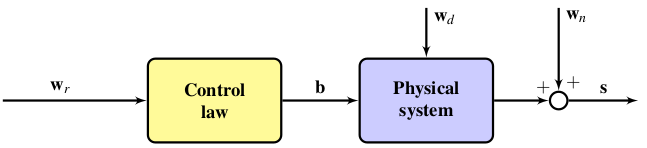
\includegraphics[width=12cm,origin=c]{Imagenes/open_loop.png}
            \caption{\textbf{Fig. 1} Open-Loop Control System, siendo $\mathbf{w_r}$ la señal de referencia, \textbf{b} la señal de
            actuación, $\mathbf{w_d}$ perturbaciones externas, $\mathbf{w_n}$ ruido introducido por los sensores involucrados y
            \textbf{s} la señal de salida. Imagen tomada de \cite{Duriez2016}} \label{fig001}
        \end{figure}

        \begin{figure}[!Hhtb]
            \centering
            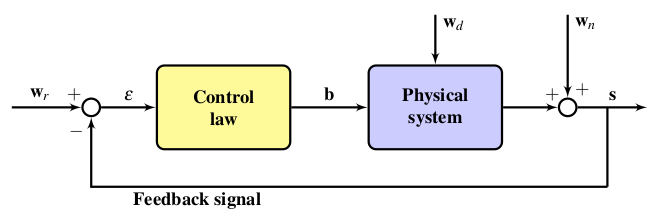
\includegraphics[width=12cm,origin=c]{Imagenes/closed_loop.png}
            \caption{\textbf{Fig. 2} Closed-Loop Control System, siendo $\mathbf{w_r}$ la señal de referencia, \textbf{b} la señal
            de actuación, $\bm{\varepsilon}$ la función de error, $\mathbf{w_r}$ perturbaciones externas, wn ruido introducido por los
            sensores involucrados y \textbf{s} la señal de salida. Imagen tomada de \cite{Duriez2016}} \label{fig002}
        \end{figure}

        Si bien los sistemas de control a lazo cerrado son complejos de diseñar y mantener, son los únicos que permiten estabilizar
        aquellos sistemas físicos que se ven afectados por estímulos externos. Esto último no es posible de realizar en un sistema de
        lazo abierto. Es por esta razón que este tipo de modelo es el mayormente usado para resolver problemas de naturaleza compleja
        (no lineales, caóticos, etc.) con un alto grado de interacción con variables externas.
        \indent Diseñar la ley de control que logre estabilizar el sistema deseado es un reto. Esto se debe a que, además de tener una
        comprensión matemática del sistema físico, se deben tener en cuenta todas las variables externas que modifican al mismo. Por esta
        razón, es importante tener una medida de la calidad de la ley de control propuesta. En la figura \label{fig003} se muestra un
        sistema a lazo cerrado con la adición de una función de costo \textbf{J}. Esta función de costo es la clave para lograr definir
        luego un método efectivo para encontrar leyes de control a través del MLC.

        \begin{figure}[!Hhtb]
            \centering
            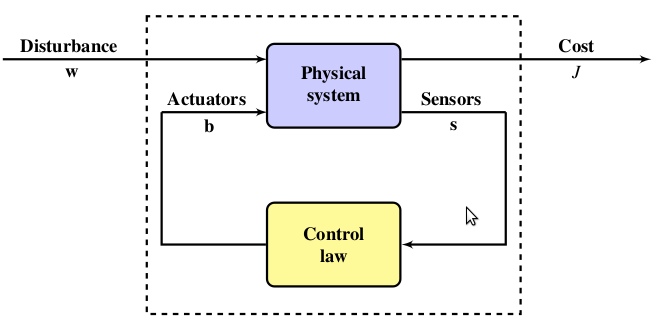
\includegraphics[width=12cm,origin=c]{Imagenes/control_loop.png}
            \caption{\textbf{Fig. 3} Sistema de Control a Lazo Cerrado de Costo \textbf{J}.
            Imagen tomada de \cite{Duriez2016}} \label{fig003}
        \end{figure}

        \subsection{Motivación} \label{sec:motiv}
        La estabilización de flujos turbulentos es una de las ramas más estudiadas dentro del control de fluídos. Las
        dificultades presentes en la resolución de este tipo de problemas, sumado a la gran cantidad de campos de aplicación, hacen del
        mismo un tema atractivo para científicos alrededor del mundo. Se listan a continuación algunas de las características más
        importantes:

        \begin{itemize}
            \item La cantidad de grados de libertad (debido a la naturaleza no lineal y caótica de los mismos) \textbf{dificulta la
            modelización del sistema físico}
            \item La naturaleza no lineal de esta clase de flujos impide aplicar el principio de superposición sobre los efectos producidos
            por cada actuador.
            \item Perturbaciones externas como el \textbf{impiden encontrar una ley de control que lleve a la
            convergencia del sistema}, aún cuando se haya realizado una correcta modelización del mismo.
            \item Los flujos turbulentos poseen \textbf{estabilidad estacionaria} (existen valores definidos para variables estadísticas
            como la media y varianza). Esto permite que el sistema vuelva a su estado original luego de ser estimulado, haciendo posible
            la reproducibilidad de los experimentos a realizar.
        \end{itemize}

        Teniendo en cuenta las características enumeradas, el campo de los fluídos turbulentos permite encontrar leyes de control válidas
        basadas en prueba y error. Esto fue lo que motivó el desarrolló del framework MLC, el cual se describe a continuación.

    \subsection{MLC} \label{sec:mlc}
    \subsubsection{Arquitectura}
        MLC es un framework utilizado para descubrir leyes de control. Tiene como fin generar modelos de sistemas de forma automática,
        los cuales llamaremos controladores, a través de información de la calidad de la solución generada. Esta información es procesada
        a través de métodos basado en \textit{Machine Learning}, los cuales están diseñados para buscar nuevos controladores dentro del
        espacio de soluciones existente. La arquitectura básica del mismo se exhibe en la figura \ref{fig004}.

        \begin{figure}[!Hhtb]
            \centering
            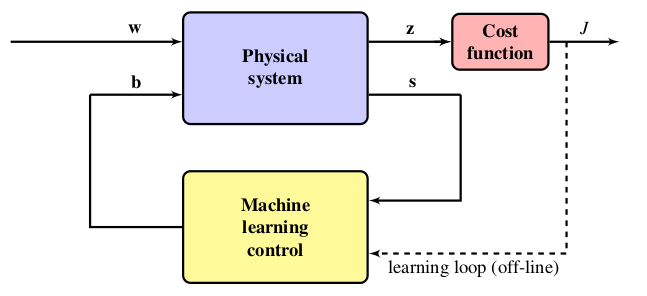
\includegraphics[width=12cm,origin=c]{Imagenes/MLC_architecture.png}
            \caption{\textbf{Fig. 4} Arquitectura del MLC. Imagen tomada de \cite{Duriez2016}} \label{fig004}
        \end{figure}

        \indent Comparando las figuras \ref{fig003} y \ref{fig004}, se puede observar como la ley de control es reemplazada por el MLC, 
        el cual recibe como entrada los valores sensados \textbf{s} y un costo asociado a la ley de control, resultante de la aplicación 
        de la función de costo \textbf{J} ante la salida del sistema físico excitado. En función de estas muestras, MLC genera una nueva 
        ley de control con el objetivo de \textit{minimizar/maximizar} el resultado de la evaluación de la función de costo 
        \textbf{J}.

        \indent La \textit{función de costo} debe ser definida por el usuario del MLC. La misma debe adecuarse al tipo de problema que se 
        desea resolver. Se puede pensar como ejemplo la estabilización de un flujo turbulento: se puede considerar que el sistema converge 
        si la velocidad del mismo en diferentes puntos es semejante (deja de ser turbulento para pasar a ser laminar). Una 
        \textit{función de costo} válida en este contexto sería aquella que arroje un número que tienda a cero en cuanto las velocidades 
        tienden a ser homogéneas.
        

    \subsubsection{Machine Learning y Programación Genética} \label{sec:mlc_and_gp}
        \textbf{Machine Learning} es una subrama de las ciencias de la computación basada en las campos de \textit{Pattern Recognition} y
        \textit{Computational Learning Theory}. La misma es utilizada, entre otros usos, para identificar sistemas dentro de un espacio de
        soluciones de alta dimensionalidad (\textit{high dimensional search space}) a través de técnicas de aprendizaje. Existe una gran
        cantidad de técnicas a utilizar dentro del campo de \textbf{Machine Learning}, tales como \textit{Gradient Search} o
        \textit{Monte-Carlo Statistical Analysis}, pero las mismas poseen como característica principal la obtención de soluciones
        subóptimas o asociadas con un costo alto cuando el espacio de soluciones es extremadamente grande \cite{Duriez2016}. Es aquí
        donde entran en juego los algoritmos
        evolucionarios, los cuales han demostrado ser óptimos a la hora de resolver este tipo de problemas. \\

        \indent La \textit{Programación Genética} y los \textit{Algoritmos Genéticos} se basan en la propagación de generaciones de
        individuos, llamadas poblaciones, los cuales son seleccionados en función del resultado de la evaluación de una 
        \textit{función de costo} \textbf{J}, también llamada \textit{función de fitness}. Dicho resultado es conocido como \textit{costo}
        o \textit{fitness}. 
        Un individuo en este ámbito \textit{tiene una correspondencia directa con la estructura y parámetros que definen
        a una ley de control}. En la figura \ref{fig005} se exhibe un diagrama detallado del uso de estos algoritmos dentro de la solución
        implementada en MLC. Un individuo $\mathbf{b = K(s)}$ es evaluado en el sistema dinámico. De dicha evaluación, se obtiene su
        \textit{fitness}. Al terminar de evaluar una población entera, MLC genera una nueva población a través del uso de
        diferentes técnicas de \textit{Programación Genética}. Este proceso se exhibe en detalle en la sección \ref{sec:law_gen}. \\

        \begin{figure}[!Hhtb]
            \centering
            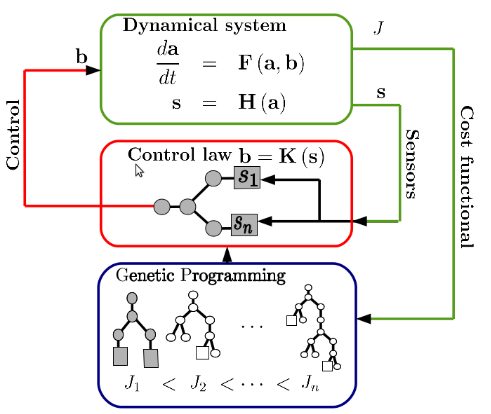
\includegraphics[width=9cm,origin=c]{Imagenes/MLC_block_diagram.png}
            \caption{\textbf{Fig. 5} Generación de nuevas leyes de control. Imagen tomada de \cite{Duriez2016}} \label{fig005}
        \end{figure}

        Un individuo se encuentra modelizado dentro del MLC como un conjunto de funciones y parámetros que poseen la forma de un
        \textit{recursive function tree}. Las funciones matemáticas utilizadas son las operaciones +, -, $\times$, / con el agregado
        de cualquier otro tipo de función, como puede llegar a ser un coseno, una exponencial o una tangente hiperbólica por nombrar
        algunas. Los nodos hojas poseen constantes o bien parámetros del sistema (por lo general sensores), mientras que los nodos no hoja
        poseen las funciones matemáticas anteriormente nombradas. La figura \ref{fig006} muestra la modelización de un individuo.
        La composición de los individuos a través de \textit{trees} hacen de los mismos candidatos ideales para ser utilizados como input
        dentro de \textit{algoritmos genéticos}.

        \begin{figure}[!Hhtb]
            \centering
            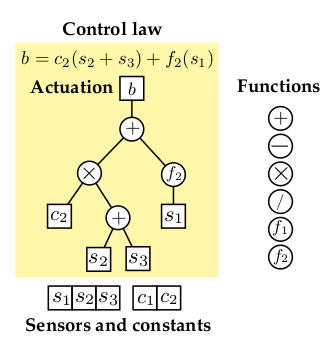
\includegraphics[width=6cm,origin=c]{Imagenes/individual_tree.png}
            \caption{\textbf{Fig. 6} Individuo $\mathbf{b = K(s_1, s_2, s_3)}$ visto como un \textit{recursive funcion tree}. Imagen
            tomada de \cite{Duriez2016}} \label{fig006}
        \end{figure}


    \subsubsection{Generación de nuevas Leyes de Control} \label{sec:law_gen}
        \indent La primera población de individuos es generada de forma aleatoria en función de los sensores, constantes y funciones
        matemáticas a disposición y la misma no posee un costo asociado a priori. La población luego es evaluada. Este proceso consiste en 
        tomar muestras de los sensores involucrados en la ley de control y reemplazarlas en la función matemática que define a un 
        individuo. De dicha evaluación se obtiene el \textit{fitness} asociado a cada individuo. A partir de
        este punto se procede a evolucionar la población. Dicha evolución se lleva a cabo a través de los siguientes algoritmos
        \cite{Duriez2016}:

        \begin{itemize}
            \item \textbf{Elitismo:} Se eligen a los mejores individuos de la población evaluada y se agregan directamente en la próxima
            generación.
            \item \textbf{Replicación:} De forma aleatoria, se eligen algunos individuos de la población evaluada y se hace avanzar a los
            mismos a la próxima población.
        \item \textbf{Crossover:} Se toman a dos individuos que posean un \textit{fitness} similar y se intercambian de forma aleatoria
            algunas ramas del \textit{recursive tree} asociado a cada uno.
            \item \textbf{Mutación:} Se modifican de forma aleatoria los parámetros o funciones de ciertos individuos.
        \end{itemize}

        Luego de realizar la evolución de la población se procede nuevamente a evaluar a la misma. A partir de este momento, ese proceso
        se repite hasta que se llega a algún punto de corte. Por lo general, el punto de corte del algoritmo utilizado por MLC consiste
        en la cantidad de generaciones evaluadas y evolucionadas hasta el momento. Otro punto de corte que se puede utilizar es haber
        alcanzado algún \textit{fitness} deseado en el mejor individuo. En la figura \ref{fig007} se muestra un diagrama de flujo
        explicando el proceso de generación de nuevas poblaciones.

        \begin{figure}[!Hhtb]
            \centering
            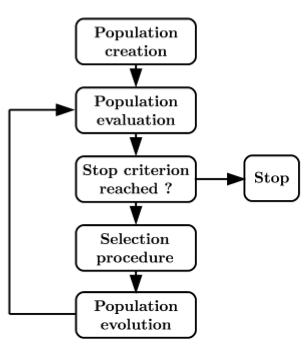
\includegraphics[width=6cm,origin=c]{Imagenes/flow_diagram.png}
            \caption{\textbf{Fig. 7} Diagrama de Flujo del proceso de Generación de Poblaciones.
            Imagen tomada de \cite{Duriez2016}} \label{fig007}
        \end{figure}

    \newpage
    \section{Objetivo}
        Durante los años que Thomas ha estado trabajando en MLC se ha encontrado con una serie de dificultades técnicas y
        funcionales. Durante el segundo cuatrimestre del 2015, como parte de un trabajo práctico de la asignatura \textit{75.61 Taller de
        Programación III} se trabajó sobre el sistema MLC, relevando requerimientos e implementando en forma parcial alguno de ellos.
        Debido al corto período tiempo dispuesto en la asignatura y la cantidad de tareas a realizar, se decidió continuar con el mismo
        como parte del presente Trabajo Profesional. Con más recursos a disposición y luego de diferentes reuniones que hemos tenido con
        Thomas, se llegó a una lista de objetivos en común. La misma se exhibe a continuación:

        \begin{itemize}
            \item \textbf{Migrar el sistema de MATLAB a Python:} MLC se encuentra desarrollado enteramente en MATLAB, con excepción del
            código que es utilizado en los dipositivos \textit{Arduino}. Las principales razones por las cuales se desea realizar esta
            migración son:
            \begin{itemize}
                \item Gracias a la cantidad de bibliotecas científicas robustas que dispone el lenguaje (\textit{numpy, matplotlib,
                SciPy Stack, etc.}), Python permite desarrollar aplicaciones de procesamiento numérico y matemático de 100\% Open
                Source
                \item Si bien MATLAB es el lenguaje más utilizado en la comunidad científica, no es un buen
                lenguaje para diseñar aplicaciones de software complejas. Entre las principales desventajas que posee, se pueden listar
                el limitado soporte a OOP (\textit{Object Oriented Programming}) y estructuras de datos y sintaxis a medida para el
                procesamiento de matrices.
            \end{itemize}

            \item \textbf{Pruebas unitarias, de integración y funcionales:} El software no posee ningún tipo de testing. Hoy en día el
            correcto funcionamiento del software es validado de forma manual por Thomas. Es de interés
            MLC es de interés agregar tests que permitan tener una medida de la cobertura de código alcanzada, como así definir métricas
            automáticas que permitan a futuro ponderar la calidad del sistema.
            \item \textbf{Refactorización de Código:} Gran cantidad del proyecto se encuentra realizado con las herramientas que MATLAB
            brinda a nuestra disposición. La migración a Python abre la posibilidad de cambiar el diseño actual del sistema por uno más
            flexible y robusto.
            \item \textbf{Cuellos de Botella:} Actualmente la forma en la evalúan los individuos (o su equivalente, \textit{Control Laws})
            es poco flexible. El procedimiento implica reprogramar los dispositivos \textit{Arduino} ante cada población a ser evaluada.
            Esto último es llevado a cabo por temas de \textit{performance}, debido a que ha sido imposible para Thomas evaluar cada
            individuo por separado. Se desea identificar y reproducir las limitaciones encontradas por Thomas y encontrar soluciones a
            las mismas, siempre que estas existan.
            \item \textbf{Interfaz Gráfica:} MLC no posee interfaz gráfica alguna. Se desea crear una interfaz de escritorio
            con una correcta usabilidad que permita a usuarios de la comunidad científica aprovechar al máximo las virtudes del presente
            framework.
        \end{itemize}

    \newpage
    \section{Alcance}
    \subsection{Requerimientos Funcionales} \label{sec:functional}
        \begin{itemize}
            \item Migrar el sistema completo de \textit{MATLAB} a \textit{Python} a través de un modo de trabajo vertical. Esto implica
            ir reemplazando código \textit{MATLAB} a \textit{Python} de forma gradual, verificando en cada paso el correcto funcionamiento
            del sistema.
            \item Utilizar el MLC desde Python con \textit{Simulink} de forma opcional. Debido a que gran cantidad de los experimentos
            realizados por \textit{Thomas} son diseñados en \textit{Simulink}, y dado que no existe una reemplazo a esta herramienta, se
            debe respetar esta compatibilidad.
            \item Diseñar e implementar un modelo de persistencia de la aplicación basado en Base de Datos. En estos momentos los datos
            de las simulaciones realizadas se almacenan en formato binario. Se debe permitir poder manipular varios experimentos a la vez
            sin la necesidad de estar cambiando los archivos de configuración como se está realizando actualmente.
            \item Rediseñar el procesamiento de las leyes de control. Esto es lo que actualmente se está realizando de forma desprolija
            en el \textit{Arduino}
            \item Diseñar e implementar un protocolo de comunicación que permita configurar y evaluar las leyes de control. Esto implica
            transformar los individuos de un \textit{recursive function tree} a un formato que pueda interpretado por los dispositivos
            \textit{Arduino} u otro dipositivo que respete el protocolo en cuestión. Se debe evitar, siempre que se pueda lograr, tener
            que quemar el \textit{Arduino} en cada iteración.
            \item Desarrollar una API genérica que permita comunicar al sistema MLC con el sistema embebido. De esta forma se busca
            desacoplar al sistema en su totalidad de algún dispositivo de hardware específico, dejando abierta la posibilidad de poder
            cambiar el mismo por alguna otra plaqueta (Raspberry, beagleboard, etc.) en un futuro.
            \item Implementar una interfaz gráfica que permita configurar los parámetros de entrada del sistema.
            \item Implementar una interfaz gráfica para la visualización y el análisis de los resultados de las simulaciones realizadas.
        \end{itemize}

    \subsection{Requerimientos No Funcionales} \label{sec:no_functional}
        \begin{itemize}
            \item El sistema debe ser multiplataforma y debe estar implementado con tecnologías de \textit{Open Source}. Una excepción a
            esto es el uso de \textit{Simulink}, como se explicó en la sección \ref{sec:functional}.
            \item Se debe evaluar que la velocidad de procesamiento de cada individuo \textit{control law} sea menor al tiempo de actuación 
            del sistema físico luego de la refactorización. En caso de no cumplirse este objetivo, se debe utilizar el esquema de trabajo 
            actual y pensar en futuras implementaciones y tecnologías que permitan resolver este problema.
            \item Generar un set de pruebas de integración que permitan validar el funcionamiento del sistema con el cliente.
            \item Implementar un conjunto de test unitarios que garanticen la cobertura de código de los módulos del sistema de acuerdo
            a las métricas de calidad definidas.
            \item Relevar qué métricas se están usando en el laboratorio para medir la performance y qué números está manejando Thomas en
            este momento.
            \item Realizar un estudio de mercado sobre las tecnologías embebidas comerciales existentes, de forma de encontrar el producto
            óptimo que cumpla con la relación velocidad de comunicación / precio. Uno de los objetivos que se busca a través del MLC, es
            lograr que los dispositivos físicos a utilizar para el sensado de parámetros y actuación sea barato y fácil de conseguir
            en cualquier parte del mundo.
        \end{itemize}

    \newpage
    \section{Especificaciones del Sistema}
    \subsection{Hardware}
    \subsubsection{MLC}
        MLC no posee limitaciones de hardware conocidas. Por esta razón, se toma como mínimo hardware requerido para ejecutar la
        aplicación el mínimo requerido por un sistema Unix. Los requerimientos mínimos se listan a continuación:

        \begin{itemize}
            \item Procesador x86 de 1 GHZ
            \item 512 MB RAM (1 GB recomendado)
            \item 20 GB de espacio en disco (la mayoría de este espacio está destinado a la instalación del MATLAB. En un futuro cuando
                se remueva la dependencia con MATLAB podrá reducirse este número, siempre y cuando no se utilice $\mathit{Simulink}$)
        \end{itemize}

    \subsubsection{Sensado y Actuación}
        Los dispositivos utilizados para realizar el sensado de magnitudes físicas y la actuación de dispositivos físicos son
        \textit{Arduinos}. El modelo utilizado del mismo no ha sido definido aún, pero se están realizando con pruebas con el modelo
        \textit{Due}. Es posible que este modelo se cambie por otro \textit{Arduino} o por otro dispositivo embebido que cumpla con los
        requerimientos necesarios.

    \subsection{Software}
    \subsubsection{MLC}
        En su versión terminada, el sistema correrá enteramente en \textbf{Python 2.7}. Se utilizarán todas las bibliotecas matemáticas
        necesarias para reemplazar la funcionalidad de MATLAB en Python. A priori, se supone que con el conjunto provisto por el
        \textit{Scipy Stack} debería ser suficiente, pero no se descarta tener que agregar alguna otra dependencia al proyecto. \\
        \indent Para realizar la migración a Python, se utilizará el módulo \textit{Python Engine}. El mismo permite ejecutar código
        MATLAB en Python. Este módulo es provisto por MATLAB a partir de la versión \textbf{R2014 B}. Como se bien se ha comentado, en su
        versión final MATLAB no será necesario para utilizar MLC, pero existen algunas herramientas provistas por \textit{Mathworks} como
        \textit{Simulink} que no poseen un reemplazo. Por esta razón es que se agrega como una de las dependencias de software a MATLAB. \\
        \indent Aún no se ha decidido que framework gráfico será utilizado para realizar la interfaz gráfica de la aplicación. Se debe
        evaluar entre las diferentes versiones disponibles para Python (PyQT4, PyQT5, Pyside, PyGTK, wxWidgets, etc.) y elegir la que sea
        más conveniente. \\
        \indent En lo que respecta a base de datos, tampoco se ha decidido aún que motor se utilizará. Debido a que el volumen de datos
        manejados por experimento es baja (cota superior de 500 MB) se analizará utilizar algún motor ligero como SQLite. En caso que se
        necesite un motor más robusto, se analizará el uso de otras opciones como pueden llegar a ser MySQL, Postgres, MariaDB o algún tipo
        de motor No SQL.

    \subsubsection{Sensado y Actuación}
        El software utilizado para el desarrollo de los dispositivos embebidos está fuertemente atado al SDK liberado por cada fabricante.
        En el caso de \textit{Arduino}, los mismos proveen un IDE que viene integrado con un cross-compiler compatible con el hardware
        disponible en cada una de las placas a disposición (\textit{Arduino Uno, Due, Mega, etc.}). Habiendo dicho esto, todo el desarrollo
        con \textit{Arduino} se realizará en C y C++.

    \newpage
    \section{Metodología}
        La metodología de trabajo elegida para trabajar en el proyecto es \textit{Scrum}. El uso de esta metodología es ideal para el tipo
        de desarrollo a realizar, debido a que se posee un cliente real con el cual trabajar. La duración de cada uno de
        los sprints variará entre dos y tres semanas. En la finalización de cada sprint, se realizará una demo con el cliente mostrando 
        los avances realizados. \\
        \indent Se utilizará \textbf{Trello} como herramienta de gestión de proyecto. En el mismo se encontrará el \textit{backlog} y
        cada uno de los \textit{sprints} realizados durante el transcurso del proyecto. A través de los plugins \textbf{Ollert} y
        \textbf{BurndownChartForTrello} se mantendrá el registro de las horas trabajadas en cada tarea, así como también se tomarán
        estadísticas de la eficiencia del equipo de trabajo. \\
        \indent El hosting del proyecto se encontrará en un repositorio privado por pedido expreso de Thomas. Al finalizar el presente
        trabajo se liberará el código a la comunidad. El hosting utilizado actualmente es \textbf{www.github.com}, y el mismo se utilizará
        además para mantener trazabilidad entre las tareas definidas en \textbf{Trello} y las modificaciones de código realizadas.



    \newpage
    \section{Cronograma}
        La asignatura \textit{75.99 Trabajo Profesional} posee asociados 12 créditos en el plan de estudios de la carrera Ingeniería en
        Informática. Esto impĺica que, según el estatuto de la facultad, la misma posee una carga horaria de 24 horas semanales (12 de
        cursada + 12 horas de trabajo por cuenta del alumno). Teniendo en cuenta que la duración de un cuatrimestre es de 16 semanas,
        la cantidad de horas asignadas a cada alumno equivale a 384 horas. Este número por 3 (la cantidad de integrantes del presente
        proyecto), da como resultado el número total de horas del proyecto: 1152. Se redondea este número de horas a 1200 para realizar
        la planificación del proyecto. A continuación se define el cronograma tentativo de tareas:

        \begin{center}
        \hspace*{-1.5cm}
        \begin{longtable}{|p{3.5cm}|p{7cm}|c|}
            \hline
            \textbf{Tarea} & \textbf{Descripción} & \textbf{Horas} \\
            \hline
            Gestión de Proyecto & Seguimiento de tareas, análisis de métricas, planeamiento de sprints y
            desarrollo del proyecto & 75 \\
            \hline
            Reuniones de Avance & Tiempo dedicado a las reuniones a tener tanto con el cliente como con los tutores. Esto último incluye
            las demos a realizar en la finalización de cada \textit{sprint} & 50 \\
            \hline
            Migración algoritmos genéticos & Migrar de MATLAB a Python la generación y evolución de individuos & 200 \\
            \hline
            Diseño e Implementación del modelo de persistencia & Se debe modelar tipos de datos a fin de persistir los experimentos
            en algún esquema de base de datos a definir & 45 \\
            \hline
            Análisis e Implementación de Gráficos & Se debe analizar que herramientas provistas por Python se amoldan a los requerimientos
            gráficos de la aplicación, que incluye la implementación de los gráficos existentes & 40 \\
            \hline
            Obtención de métricas y análisis de disp. \textit{Arduino} & Se realizarán pruebas de desempeño de hardware de comunicación
            para dispositivos \textit{Arduino}, a fin de determinar la viabilidad del procesamiento de las leyes de control en Python
            & 30 \\
            \hline
            Diseño e Implementación de Protocolo de Comunicación & El protocolo debe ser capaz de configurar los sensores y actuadores
            a utilizar en un experimento dado. También debe ser capaz de obtener lecturas de los sensores previamente configurados y
            manipular los actuadores & 100 \\
            \hline
            Confección de Pruebas de Integración & Se debe generar un conjunto de pruebas que permitan validar el correcto funcionamiento
            entre las diferentes partes que componen al MLC & 30 \\
            \hline
            Diseño y Armado de Entorno de Prueba Real & Se debe implementar un experimento de laboratorio que permita evaluar el correcto
            funcionamiento y desempeño del MLC & 60 \\
            \hline
            Análisis y Diseño de Mejoras de Arquitectura & Una vez que se haya migrado el MLC a Python, se procederá a evaluar
            mejoras en el diseño del sistema & 90 \\
            \hline
            Implementación de Mejoras de Arquitectura & Con la nueva arquitectura y diseño en mente, se procederá a implementar
            la nueva solución propuesta & 270 \\
            \hline
            Documentación Interna de diseño & Documentación que describa el diseño y arquitectura del sistema. La misma debe incluir
            diagramas clases, secuencia, etc., como así también el detalle del protocolo de comunicación implementado & 60 \\
            \hline
            Diseño e Implementación de Interfaz Gráfica & Se debe desarrollar una interfaz gráfica agradable para el usuario que permita
            la administración y configuración del sistema. La misma debe incluir configurar y visualizar los experimentos a realizar
            & 30 \\
            \hline
            Implementación de Instaladores & Se deben crear instaladores para los sistemas operativos más conocidos
            (Windows, MAC, Linux flavors) con el fin de facilitar el uso del MLC en la comunidad científica & 60 \\
            \hline
            Elaboración de Manual de Usuario & Se deben confeccionar los manuales de usuario para el uso y extensión de la versión final
            del sistema & 60 \\
            \hline
            \multicolumn{2}{|c|}{\textbf{Total Horas:}} & \textbf{1200} \\
            \hline
        \end{longtable}
        \end{center}

    \newpage
    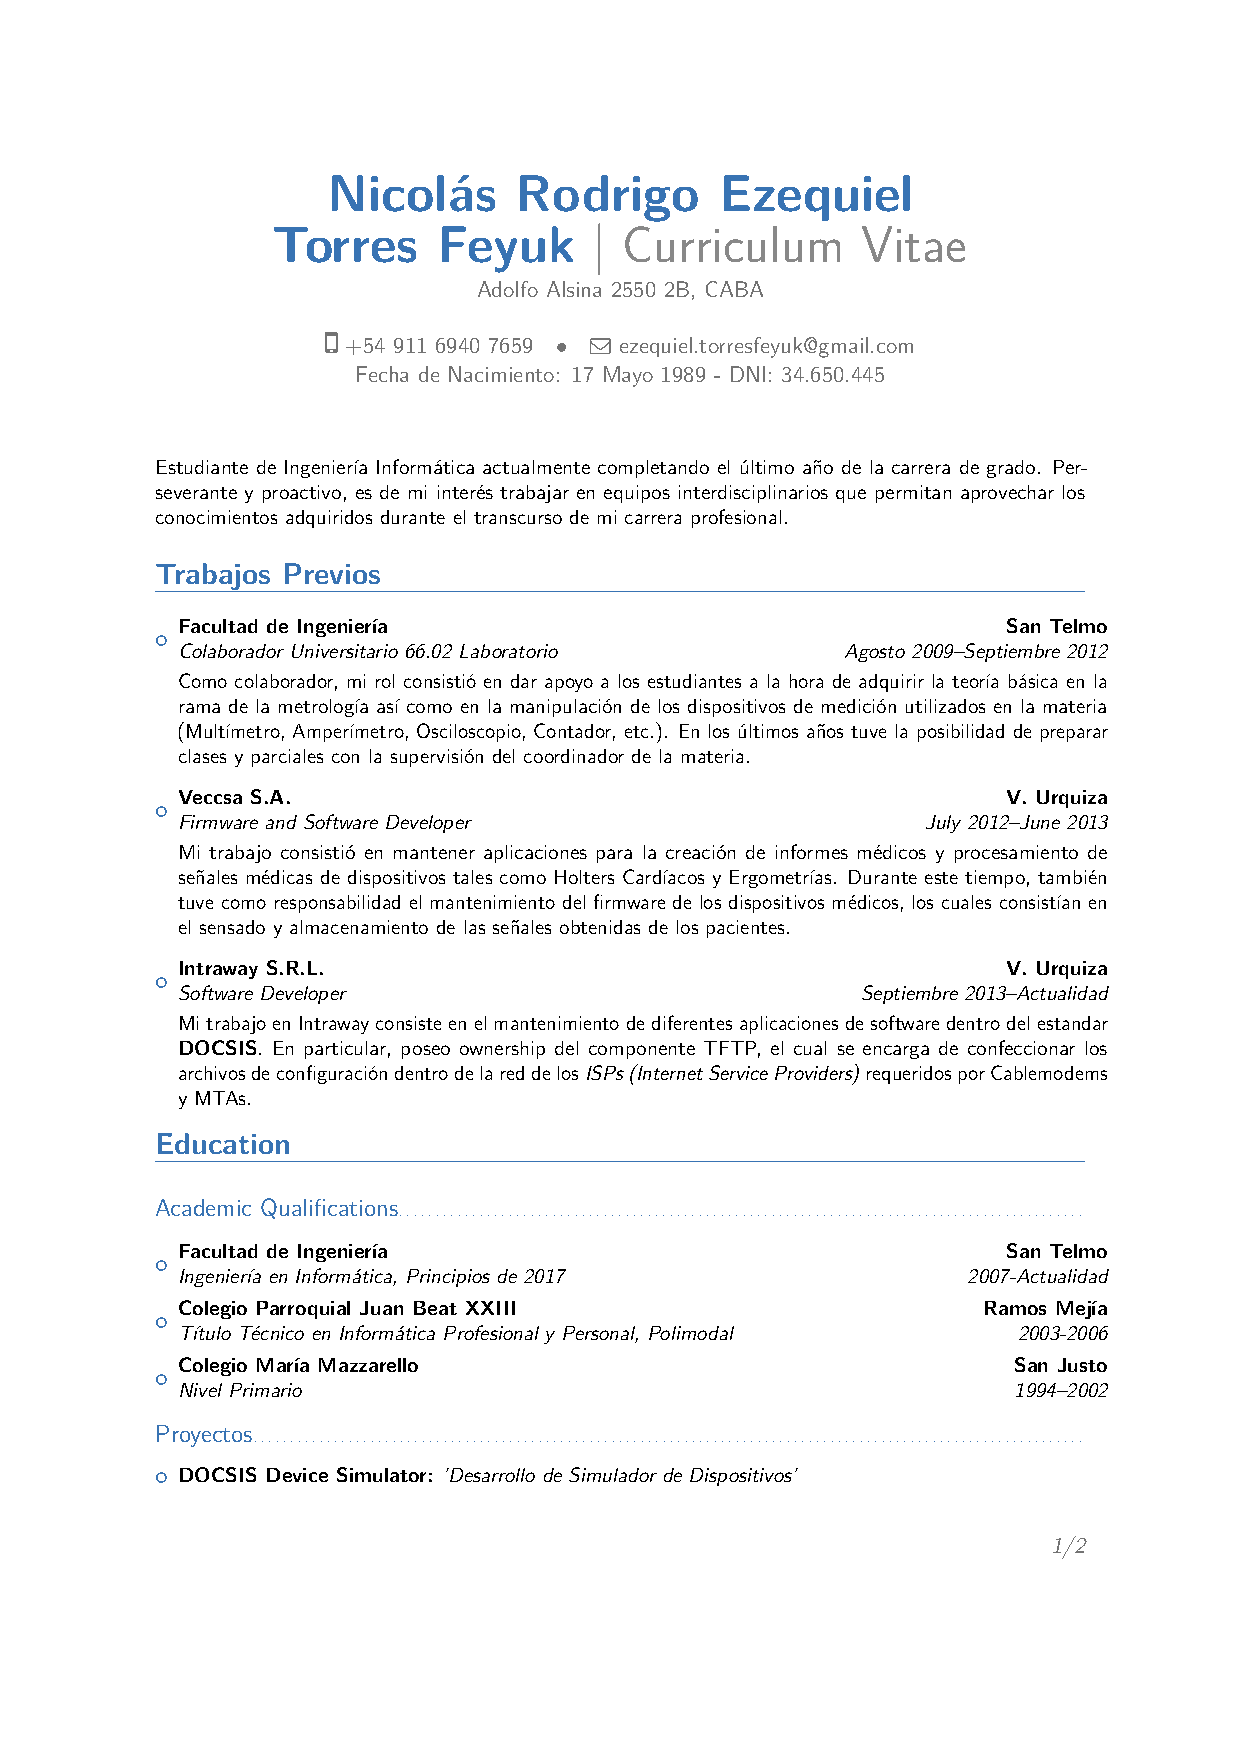
\includepdf[scale=0.8,clip,trim=0cm 0cm 0cm -3cm,pages={1},pagecommand={\section{Datos Integrantes}\subsection{Ezequiel Torres Feyuk}\subsubsection{CV}}]{CVs/TorresFeyuk/CV.pdf} 
    \includepdf[scale=0.8,clip,trim=0cm 0cm 0cm 2cm,pages={2},pagecommand={}]{CVs/TorresFeyuk/CV.pdf}

    \newpage
    \subsubsection{Listado de Materias}
            \small{
        \begin{center}
        \hspace*{-1cm}
        \begin{tabular}{|c|c|c|c|c|c|}
            \hline
            \textbf{Cód.} & \textbf{Asignatura} & \textbf{Nota} & \textbf{Acta} & \textbf{Fecha} & \textbf{Créd.} \\ 
            \hline
            75.40 & Algoritmos y Programación I                & 10 & 17-098-175 & 04/07/08 & 6 \\
            \hline
            61.08 & Álgebra II                                 & 6  & 01-150-248 & 10/07/08 & 8 \\
            \hline
            61.03 & Análisis Matemático II A                   & 7  & 01-151-234 & 06/08/08 & 8 \\
            \hline
            63.01 & Química                                    & 6  & 03-073-207 & 12/12/08 & 6 \\
            \hline
            61.09 & Probabilidad y Estadística B               & 6  & 01-155-032 & 11/02/09 & 6 \\
            \hline
            62.01 & Física I A                                 & 7  & 02-107-089 & 12/02/09 & 8 \\
            \hline
            75.41 & Algoritmos y Programación II               & 8  & 17-101-086 & 04/08/09 & 6 \\
            \hline 
            62.03 & Física II A                                & 5  & 02-107-156 & 05/08/09 & 8 \\
            \hline
            62.15 & Física III D                               & 6  & 02-108-001 & 23/12/09 & 4 \\
            \hline
            75.07 & Algoritmos y Programación III              & 8  & 17-102-210 & 29/12/09 & 6 \\
            \hline
            61.10 & Análisis Matemático III A                  & 7  & 01-149-225 & 10/02/10 & 6 \\
            \hline 
            66.70 & Estructura del Computador                  & 8  & 06-138-111 & 11/02/10 & 6 \\
            \hline
            66.02 & Laboratorio                                & 4  & 06-138-157 & 23/02/10 & 6 \\
            \hline
            75.12 & Análisis Numérico I                        & 8  & 17-104-058 & 14/07/10 & 6 \\
            \hline
            66.06 & Análisis de Circuitos                      & 7  & 06-140-063 & 23/02/11 & 10 \\
            \hline
            75.06 & Organización de Datos                      & 8  & 17-106-086 & 03/03/11 & 6 \\
            \hline
            75.42 & Taller de Programación I                   & 9  & 17-106-199 & 06/07/11 & 4 \\
            \hline
            66.20 & Organización de Computadoras               & 5  & 06-141-016 & 08/08/11 & 6 \\
            \hline
            75.08 & Sistemas Operativos                        & 10 & 17-107-158 & 11/08/11 & 6 \\
            \hline 
            71.14 & Modelos y Optimización I                   & 8  & 11-153-164 & 13/02/12 & 6 \\
            \hline
            66.74 & Señales y Sistemas                         & 7  & 06-141-187 & 17/02/12 & 6 \\
            \hline
            66.09 & Laboratorio de Microcomputadoras           & 9  & 06-142-046 & 13/07/12 & 6 \\
            \hline
            66.74 & Procesos Estocásticos                      & 6  & 06-142-131 & 06/08/12 & 6 \\
            \hline
            75.59 & Técnicas de Programación Concurrente I     & 6  & 17-110-020 & 08/08/12 & 6 \\
            \hline
            75.09 & Análisis de la Información                 & 5  & 17-110-135 & 10/12/12 & 6 \\
            \hline
            75.43 & Introducción a los Sistemas Distribuidos   & 8  & 17-111-028 & 28/12/12 & 6 \\
            \hline
            75.26 & Simulación                                 & 8  & 17-111-048 & 06/02/13 & 6 \\
            \hline
            75.10 & Técnicas de Diseño                         & 6  & 95-0001028 & 08/07/13 & 6 \\
            \hline
            66.08 & Circuitos Electrónicos I                   & 7  & 86-0001011 & 10/07/13 & 8 \\
            \hline
            75.15 & Base de Datos                              & 7  & 95-0001331 & 07/08/13 & 6 \\
            \hline
            75.52 & Taller de Programación II                  & 5  & 95-0002383 & 04/02/14 & 4 \\
            \hline 
            75.74 & Sistemas Distribuídos I                    & 5  & 96-0001462 & 06/02/14 & 6 \\
            \hline
            71.40 & Leg. y Ej. Prof. de la Inf. en Informat.   & 5  & 71-0001509 & 21/02/14 & 4 \\
            \hline
            71.12 & Estructura de las Organizaciones           & 6  & 71-0001490 & 26/02/14 & 6 \\
            \hline
            75.67 & Sist. Autom. De Diag. y Detec. de Fallas I & 7  & 95-0002261 & 04/08/14 & 6 \\
            \hline
            75.65 & Manufactura Integrada por Comp. (CIM) I    & 7  & 95-0002365 & 14/08/14 & 6 \\
            \hline
            75.68 & Sist. De Soporte P/Celdas de Prod. Flexib. & 10 & 95-0002440 & 10/12/14 & 4 \\
            \hline
            75.66 & Manufactura Integrada por Comp. (CIM) II   & 8  & 95-0002462 & 11/12/14 & 6 \\
            \hline
            64.05 & Estática y Resistencia de los Materiales B & 8  & 64-0001643 & 09/02/15 & 6 \\
            \hline
            75.61 & Taller de Programación III                 & 8  & 95-0003741 & 25/02/16 & 6 \\
            \hline
            \multicolumn{5}{|c|}{\textbf{Total Créditos}} & \textbf{244} \\
            \hline
        \end{tabular}
        \end{center}
    }


    \newpage
    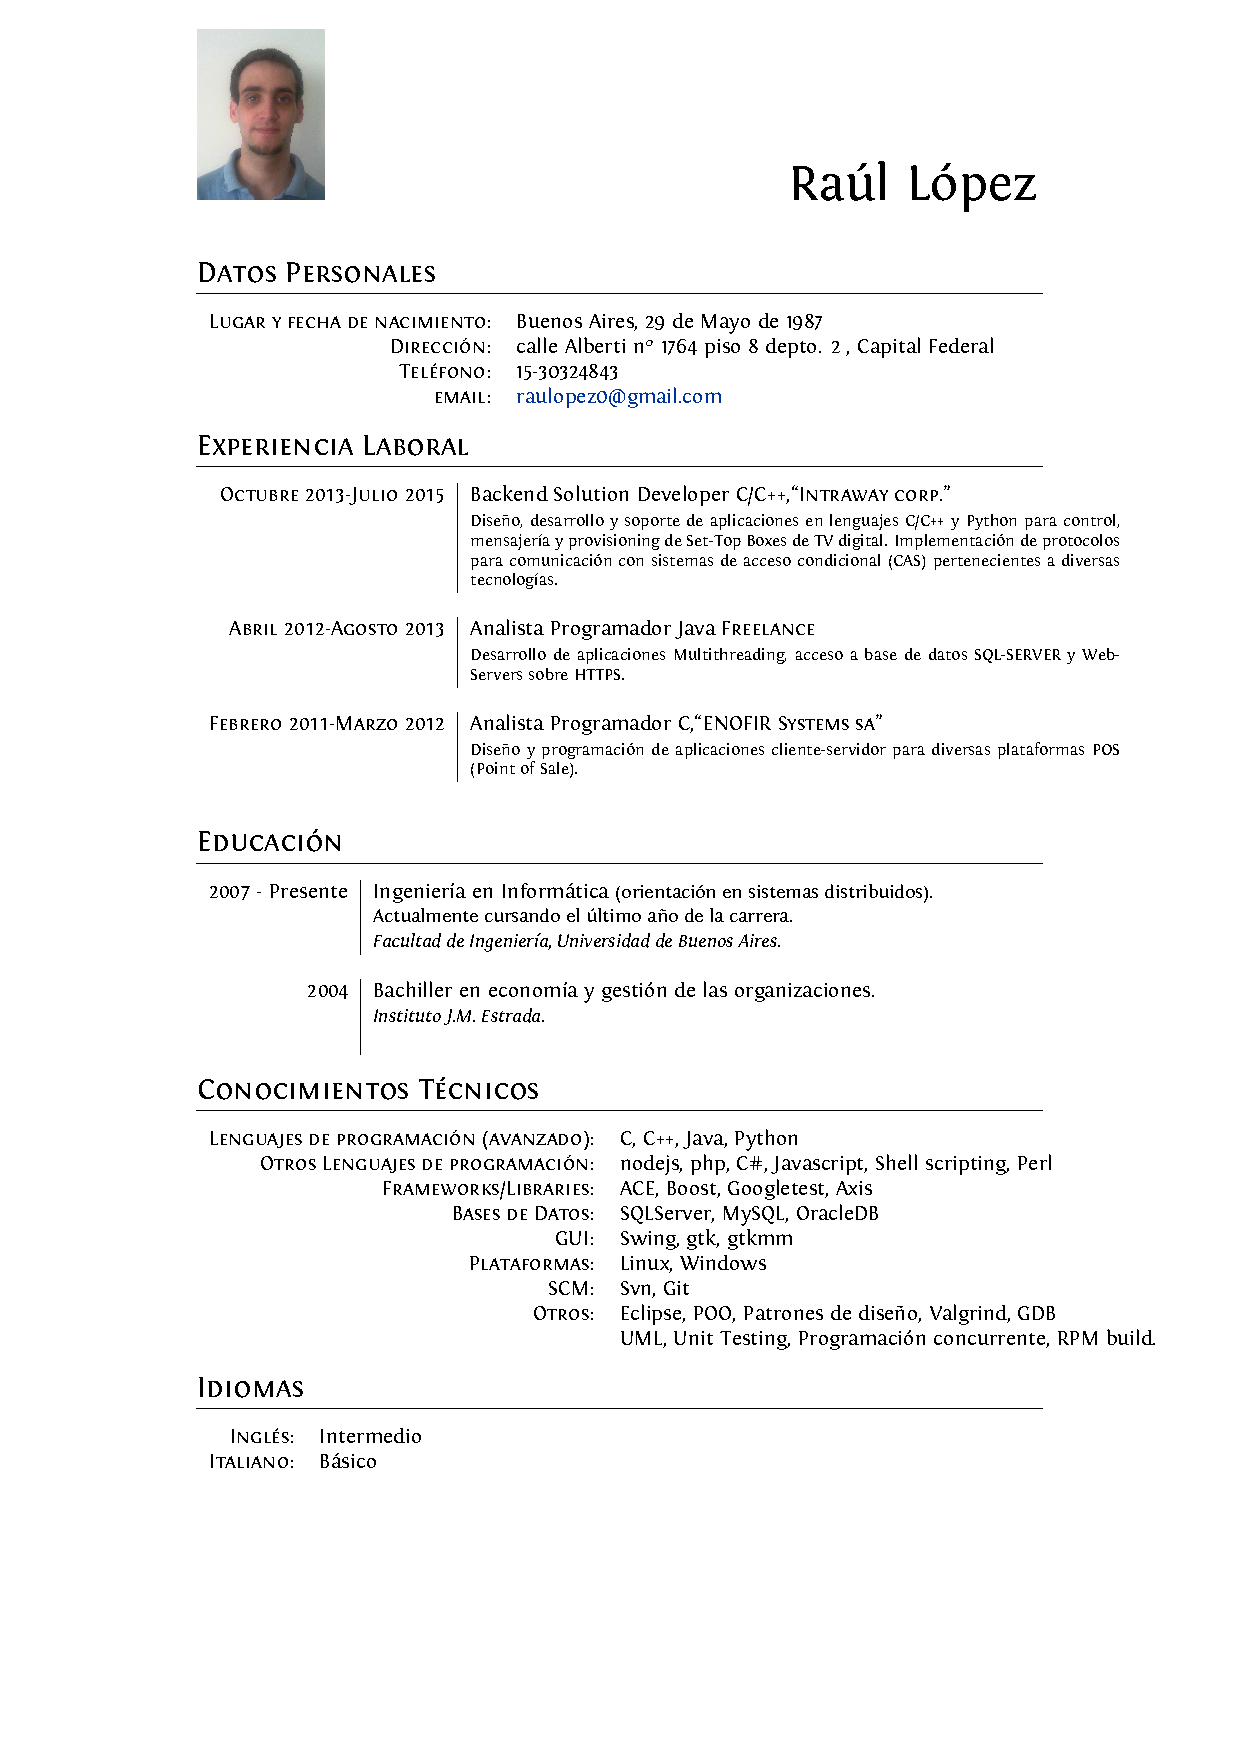
\includepdf[scale=0.8,clip,trim=0cm 0cm 0cm -5cm,pages={1},pagecommand={\subsection{Raúl Lopez Skuba}\subsubsection{CV}}]{CVs/LopezSkuba/CV.pdf} 

    \newpage
    \subsubsection{Listado de Materias}
            \small{
        \begin{center}
        \hspace*{-1cm}
        \begin{tabular}{|c|c|c|c|c|c|}
            \hline
            \textbf{Cód.} & \textbf{Asignatura} & \textbf{Nota} & \textbf{Acta} & \textbf{Fecha} & \textbf{Créd.} \\ 
            \hline
            75.40 & Algoritmos y Programación I                & 10 & 17-098-175 & 04/07/08 & 6 \\
            \hline
            61.08 & Álgebra II                                 & 6  & 01-150-248 & 10/07/08 & 8 \\
            \hline
            61.03 & Análisis Matemático II A                   & 7  & 01-151-234 & 06/08/08 & 8 \\
            \hline
            63.01 & Química                                    & 6  & 03-073-207 & 12/12/08 & 6 \\
            \hline
            61.09 & Probabilidad y Estadística B               & 6  & 01-155-032 & 11/02/09 & 6 \\
            \hline
            62.01 & Física I A                                 & 7  & 02-107-089 & 12/02/09 & 8 \\
            \hline
            75.41 & Algoritmos y Programación II               & 8  & 17-101-086 & 04/08/09 & 6 \\
            \hline 
            62.03 & Física II A                                & 5  & 02-107-156 & 05/08/09 & 8 \\
            \hline
            62.15 & Física III D                               & 6  & 02-108-001 & 23/12/09 & 4 \\
            \hline
            75.07 & Algoritmos y Programación III              & 8  & 17-102-210 & 29/12/09 & 6 \\
            \hline
            61.10 & Análisis Matemático III A                  & 7  & 01-149-225 & 10/02/10 & 6 \\
            \hline 
            66.70 & Estructura del Computador                  & 8  & 06-138-111 & 11/02/10 & 6 \\
            \hline
            66.02 & Laboratorio                                & 4  & 06-138-157 & 23/02/10 & 6 \\
            \hline
            75.12 & Análisis Numérico I                        & 8  & 17-104-058 & 14/07/10 & 6 \\
            \hline
            66.06 & Análisis de Circuitos                      & 7  & 06-140-063 & 23/02/11 & 10 \\
            \hline
            75.06 & Organización de Datos                      & 8  & 17-106-086 & 03/03/11 & 6 \\
            \hline
            75.42 & Taller de Programación I                   & 9  & 17-106-199 & 06/07/11 & 4 \\
            \hline
            66.20 & Organización de Computadoras               & 5  & 06-141-016 & 08/08/11 & 6 \\
            \hline
            75.08 & Sistemas Operativos                        & 10 & 17-107-158 & 11/08/11 & 6 \\
            \hline 
            71.14 & Modelos y Optimización I                   & 8  & 11-153-164 & 13/02/12 & 6 \\
            \hline
            66.74 & Señales y Sistemas                         & 7  & 06-141-187 & 17/02/12 & 6 \\
            \hline
            66.09 & Laboratorio de Microcomputadoras           & 9  & 06-142-046 & 13/07/12 & 6 \\
            \hline
            66.74 & Procesos Estocásticos                      & 6  & 06-142-131 & 06/08/12 & 6 \\
            \hline
            75.59 & Técnicas de Programación Concurrente I     & 6  & 17-110-020 & 08/08/12 & 6 \\
            \hline
            75.09 & Análisis de la Información                 & 5  & 17-110-135 & 10/12/12 & 6 \\
            \hline
            75.43 & Introducción a los Sistemas Distribuidos   & 8  & 17-111-028 & 28/12/12 & 6 \\
            \hline
            75.26 & Simulación                                 & 8  & 17-111-048 & 06/02/13 & 6 \\
            \hline
            75.10 & Técnicas de Diseño                         & 6  & 95-0001028 & 08/07/13 & 6 \\
            \hline
            66.08 & Circuitos Electrónicos I                   & 7  & 86-0001011 & 10/07/13 & 8 \\
            \hline
            75.15 & Base de Datos                              & 7  & 95-0001331 & 07/08/13 & 6 \\
            \hline
            75.52 & Taller de Programación II                  & 5  & 95-0002383 & 04/02/14 & 4 \\
            \hline 
            75.74 & Sistemas Distribuídos I                    & 5  & 96-0001462 & 06/02/14 & 6 \\
            \hline
            71.40 & Leg. y Ej. Prof. de la Inf. en Informat.   & 5  & 71-0001509 & 21/02/14 & 4 \\
            \hline
            71.12 & Estructura de las Organizaciones           & 6  & 71-0001490 & 26/02/14 & 6 \\
            \hline
            75.67 & Sist. Autom. De Diag. y Detec. de Fallas I & 7  & 95-0002261 & 04/08/14 & 6 \\
            \hline
            75.65 & Manufactura Integrada por Comp. (CIM) I    & 7  & 95-0002365 & 14/08/14 & 6 \\
            \hline
            75.68 & Sist. De Soporte P/Celdas de Prod. Flexib. & 10 & 95-0002440 & 10/12/14 & 4 \\
            \hline
            75.66 & Manufactura Integrada por Comp. (CIM) II   & 8  & 95-0002462 & 11/12/14 & 6 \\
            \hline
            64.05 & Estática y Resistencia de los Materiales B & 8  & 64-0001643 & 09/02/15 & 6 \\
            \hline
            75.61 & Taller de Programación III                 & 8  & 95-0003741 & 25/02/16 & 6 \\
            \hline
            \multicolumn{5}{|c|}{\textbf{Total Créditos}} & \textbf{244} \\
            \hline
        \end{tabular}
        \end{center}
    }


    \newpage
    \subsection{Marco Germano Zbrun}
    TODO: DALE MARCO, PASA EL CV!!!
    %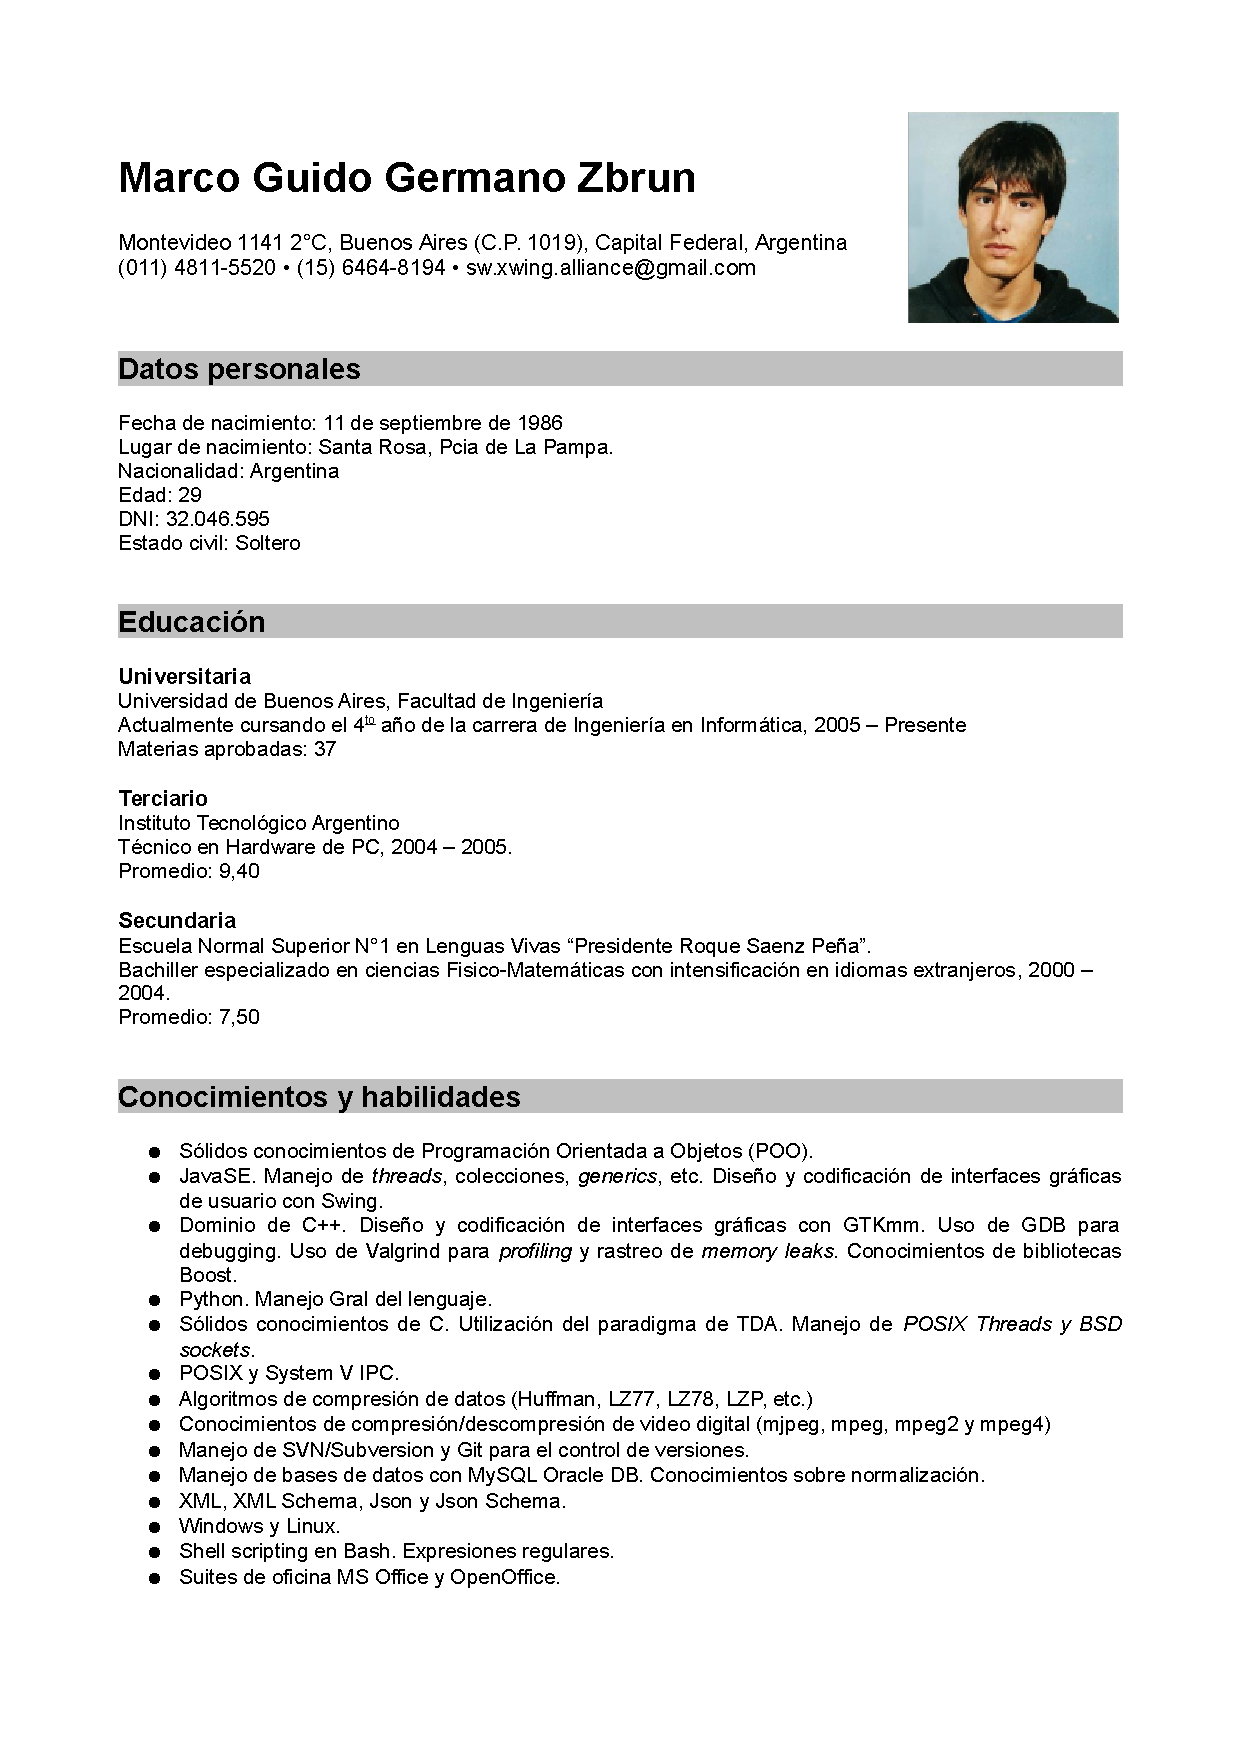
\includepdf[scale=0.8,clip,trim=0cm 0cm 0cm -5cm,pages={1},pagecommand={\section{Marco Germano Zbrun}\subsection{CV}}]{CVs/GermanoZbrun/CV.pdf} 

    \newpage
    \subsubsection{Listado de Materias}
            \small{
        \begin{center}
        \hspace*{-1cm}
        \begin{tabular}{|c|c|c|c|c|c|}
            \hline
            \textbf{Cód.} & \textbf{Asignatura} & \textbf{Nota} & \textbf{Acta} & \textbf{Fecha} & \textbf{Créd.} \\ 
            \hline
            75.40 & Algoritmos y Programación I                & 10 & 17-098-175 & 04/07/08 & 6 \\
            \hline
            61.08 & Álgebra II                                 & 6  & 01-150-248 & 10/07/08 & 8 \\
            \hline
            61.03 & Análisis Matemático II A                   & 7  & 01-151-234 & 06/08/08 & 8 \\
            \hline
            63.01 & Química                                    & 6  & 03-073-207 & 12/12/08 & 6 \\
            \hline
            61.09 & Probabilidad y Estadística B               & 6  & 01-155-032 & 11/02/09 & 6 \\
            \hline
            62.01 & Física I A                                 & 7  & 02-107-089 & 12/02/09 & 8 \\
            \hline
            75.41 & Algoritmos y Programación II               & 8  & 17-101-086 & 04/08/09 & 6 \\
            \hline 
            62.03 & Física II A                                & 5  & 02-107-156 & 05/08/09 & 8 \\
            \hline
            62.15 & Física III D                               & 6  & 02-108-001 & 23/12/09 & 4 \\
            \hline
            75.07 & Algoritmos y Programación III              & 8  & 17-102-210 & 29/12/09 & 6 \\
            \hline
            61.10 & Análisis Matemático III A                  & 7  & 01-149-225 & 10/02/10 & 6 \\
            \hline 
            66.70 & Estructura del Computador                  & 8  & 06-138-111 & 11/02/10 & 6 \\
            \hline
            66.02 & Laboratorio                                & 4  & 06-138-157 & 23/02/10 & 6 \\
            \hline
            75.12 & Análisis Numérico I                        & 8  & 17-104-058 & 14/07/10 & 6 \\
            \hline
            66.06 & Análisis de Circuitos                      & 7  & 06-140-063 & 23/02/11 & 10 \\
            \hline
            75.06 & Organización de Datos                      & 8  & 17-106-086 & 03/03/11 & 6 \\
            \hline
            75.42 & Taller de Programación I                   & 9  & 17-106-199 & 06/07/11 & 4 \\
            \hline
            66.20 & Organización de Computadoras               & 5  & 06-141-016 & 08/08/11 & 6 \\
            \hline
            75.08 & Sistemas Operativos                        & 10 & 17-107-158 & 11/08/11 & 6 \\
            \hline 
            71.14 & Modelos y Optimización I                   & 8  & 11-153-164 & 13/02/12 & 6 \\
            \hline
            66.74 & Señales y Sistemas                         & 7  & 06-141-187 & 17/02/12 & 6 \\
            \hline
            66.09 & Laboratorio de Microcomputadoras           & 9  & 06-142-046 & 13/07/12 & 6 \\
            \hline
            66.74 & Procesos Estocásticos                      & 6  & 06-142-131 & 06/08/12 & 6 \\
            \hline
            75.59 & Técnicas de Programación Concurrente I     & 6  & 17-110-020 & 08/08/12 & 6 \\
            \hline
            75.09 & Análisis de la Información                 & 5  & 17-110-135 & 10/12/12 & 6 \\
            \hline
            75.43 & Introducción a los Sistemas Distribuidos   & 8  & 17-111-028 & 28/12/12 & 6 \\
            \hline
            75.26 & Simulación                                 & 8  & 17-111-048 & 06/02/13 & 6 \\
            \hline
            75.10 & Técnicas de Diseño                         & 6  & 95-0001028 & 08/07/13 & 6 \\
            \hline
            66.08 & Circuitos Electrónicos I                   & 7  & 86-0001011 & 10/07/13 & 8 \\
            \hline
            75.15 & Base de Datos                              & 7  & 95-0001331 & 07/08/13 & 6 \\
            \hline
            75.52 & Taller de Programación II                  & 5  & 95-0002383 & 04/02/14 & 4 \\
            \hline 
            75.74 & Sistemas Distribuídos I                    & 5  & 96-0001462 & 06/02/14 & 6 \\
            \hline
            71.40 & Leg. y Ej. Prof. de la Inf. en Informat.   & 5  & 71-0001509 & 21/02/14 & 4 \\
            \hline
            71.12 & Estructura de las Organizaciones           & 6  & 71-0001490 & 26/02/14 & 6 \\
            \hline
            75.67 & Sist. Autom. De Diag. y Detec. de Fallas I & 7  & 95-0002261 & 04/08/14 & 6 \\
            \hline
            75.65 & Manufactura Integrada por Comp. (CIM) I    & 7  & 95-0002365 & 14/08/14 & 6 \\
            \hline
            75.68 & Sist. De Soporte P/Celdas de Prod. Flexib. & 10 & 95-0002440 & 10/12/14 & 4 \\
            \hline
            75.66 & Manufactura Integrada por Comp. (CIM) II   & 8  & 95-0002462 & 11/12/14 & 6 \\
            \hline
            64.05 & Estática y Resistencia de los Materiales B & 8  & 64-0001643 & 09/02/15 & 6 \\
            \hline
            75.61 & Taller de Programación III                 & 8  & 95-0003741 & 25/02/16 & 6 \\
            \hline
            \multicolumn{5}{|c|}{\textbf{Total Créditos}} & \textbf{244} \\
            \hline
        \end{tabular}
        \end{center}
    }



    \newpage
    \bibliography{mybib}{}
    \bibliographystyle{ieeetr}

\end{document}

